\documentclass[12pt]{beamer}
\usepackage{amsmath}
\usepackage[utf8]{inputenc}
\usepackage{apacite}
\usepackage[absolute,overlay]{textpos}
\usetheme{Singapore}
\usepackage[style=british]{csquotes}

\def\signed #1{{\leavevmode\unskip\nobreak\hfil\penalty50\hskip1em
		\hbox{}\nobreak\hfill #1
		\parfillskip=0pt \finalhyphendemerits=0 \endgraf}}

\newsavebox\mybox
\newenvironment{aquote}[1]
{\savebox\mybox{#1}\begin{quote}\openautoquote\hspace*{-.7ex}}
	{\unskip\closeautoquote\vspace*{1mm}\signed{\usebox\mybox}\end{quote}}

\DeclareMathOperator*{\argmin}{arg\,min}
\usepackage{soul}

\title{Does Women Care More ?}
\subtitle{The relationship between women's participation in legislation and national health expenditure\\A preliminary result }

\date{\today}
\author[author]{Zhiyuan Jiang}		
		
\begin{document}
	
\frame{\titlepage}

%-------------------------------------------------------------------------------------------------------------------------------------------------------------------------------%
%-------------------------------------------------------------------------------------------------------------------------------------------------------------------------------%
\section{Introduction and Motivation}

\begin{frame}[plain]
	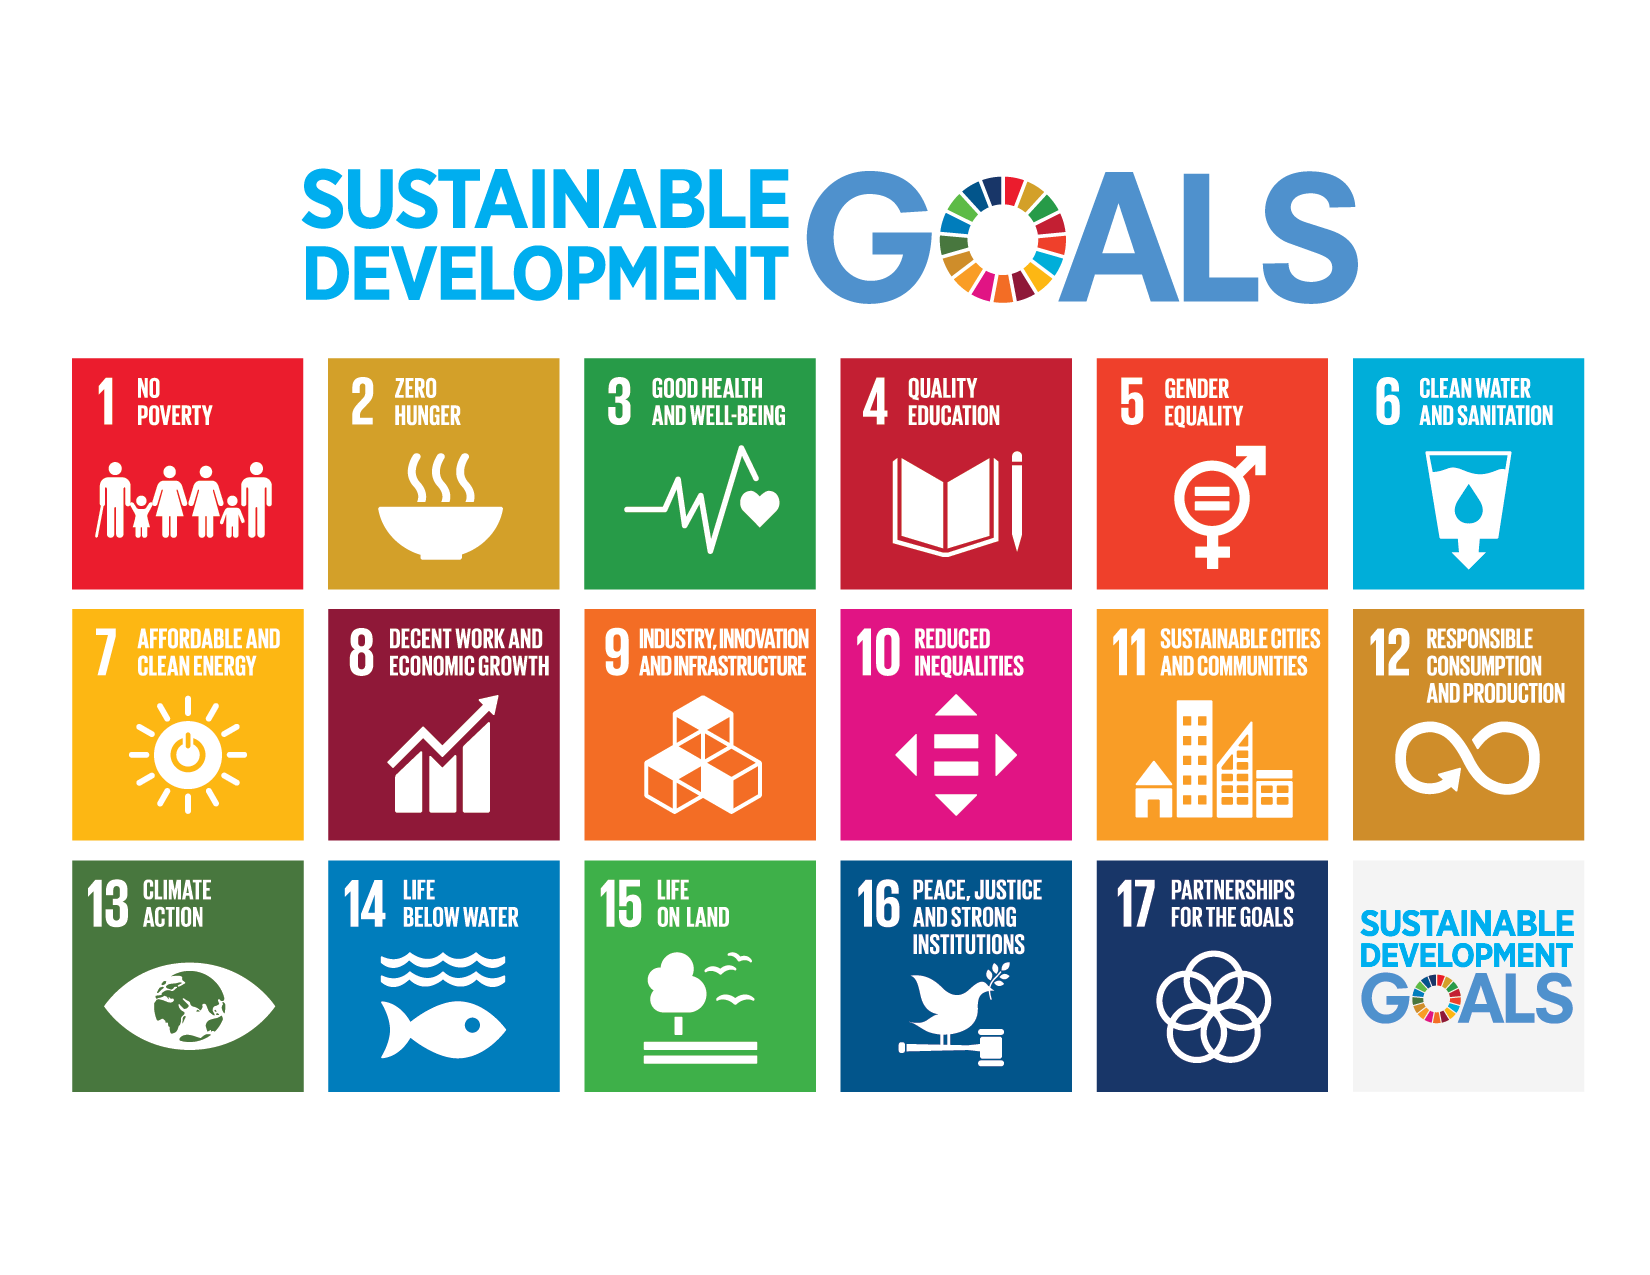
\includegraphics[scale = 0.2]{figure/SDG.png}	

\end{frame}

\begin{frame}
	\frametitle{Motivation}\pause
\begin{center}
\begin{quotation}
	"Women belong in all places where decisions are being made."
\begin{flushright}
-Ruth Bader Ginsburg
\end{flushright}
\end{quotation}
\end{center}
\end{frame}

\begin{frame}[plain]
	
\end{frame}

\begin{frame}
	\frametitle{Empowerment and Development}

	%TODO household-level research about the benefits of women empowerment
	\citeA{Duflo2012}: Survey paper supports the idea of women empowerment.\\\pause
	Empowerment and development work in both ways.\pause
	
	\begin{itemize}
		\item Empowerment relies on the development of the economy.
		\item Empowerment boosts the development of the economy. 
	\end{itemize}
\alert{Exp:} Mother's education and Children's wellbing (But biased)
\end{frame}

\begin{frame}
	\frametitle{Mechanism}
	\begin{center}
	\alert{Budget Allocation}\pause
	\end{center}
Evidences from household level:\\
\begin{itemize}
	\item \citeA{Hoddinott1995}: Studied Cote d'Ivoire. Women spend money on \alert{family friendly} items.\\
	\item \citeA{Quisumbing2003}:Cross countries study. Women spend more on \alert{education}\\
\end{itemize}
\end{frame}


\begin{frame}
	\frametitle{Influence from Politics}
	%TODO larger scale benefits
\begin{center}
	From local level government.\pause
\end{center}
	\begin{itemize}
		\item \citeA{Chattopadhyay2004}: Village council
		\item \citeA{Irma2011}: State Legislature
		\item Both studies show female politicians prefer \alert{women-friendly} decisions. Pass low on equal inheritance right, budget preference on nutrition, entry-level education etc.
	\end{itemize}
\end{frame}

\begin{frame}
	\frametitle{Even at the country level...}
	\begin{center}
		From national level government:\pause
			\end{center}
		\begin{itemize}
			\item \citeA{Dollar2001}: Corruption
			\item \citeA{Jayasuriya2013}: Economic Growth
			\item \citeA{York2014}: Life-satisfaction
			\item \citeA{Salahodjaev2020}: Deforestation
		\end{itemize}\pause
Challenger:
\citeA{Sung2003}: Better gender or better system ?
\end{frame}

\begin{frame}{Core Problem}
\pause%TODO how to transform.
\begin{center}
\alert{\textbf{Its there exist a relationship between the number of female politicans and health care budget ?}}\pause
\end{center}

Predecessors 
\begin{itemize}
\item Municipial \cite{Funk2018}
\item State \cite{Irma2011}
\item Seats Quota in parliament \cite{Chen2010}
\item $\cdots$
\end{itemize}
\end{frame}

\begin{frame}
	\frametitle{This Research}
	%TODO a more direct description of this research
	\begin{center}
		Does the ratio of female lawmakers are linked with the national health care expenditure?\\
	\end{center}
	\begin{center}
	If yes, how? \\
	If no, why?
	\end{center}
\end{frame}





%-------------------------------------------------------------------------------------------------------------------------------------------------------------------------------%



\section{Method and Data}

\begin{frame}
	\frametitle{Model: Simple}
	\begin{center}
		\begin{align*}
			HealthExp = \beta_0 + \beta_1Women\_Lawmaker\_Ratio + \boldsymbol\beta_2\mathbf{X} + \epsilon 
		\end{align*}
	\end{center}\pause
\begin{center}
	What are inside the $\mathbf{X}$ ?\\
	How to estimate the coefficient?
\end{center}

\end{frame}

\begin{frame}
	\frametitle{Data}
	\begin{enumerate}
		\item Health Care Expenditure
		\item Female Lawmaker ratio
		\item Control Variables:$\mathbf{X}$
		\item Other Indicators: Binaries
	\end{enumerate}
Use Country Level Data: 122 Countries\\
Annual data from 2001 - 2019: 20 years
\end{frame}

\begin{frame}{Data}
\frametitle{Health Care}

\begin{enumerate}
	\item The total national budget to the GDP
	\item The health care budget to the GDP
\end{enumerate}
\begin{center}
\alert{The proportion of Health Care Expenditure to the National Budget}
\end{center}

\begin{table}
\centering
\begin{tabular}{lllll} 
\hline
                     & Mean  & StD  & Min  & Max   \\ 
\hline
Global & 10.41 & 4.65 & 0.63 & 33.1  \\
High Income Countries  & 14.27 & 3.02 & 7.43 & 24.3  \\
Emerging Market & 9.55  & 3.89 & 2.62 & 18.6  \\
LDC Countries   & 6.599 & 2.27 & 1.03 & 15.0 \\
\hline
\end{tabular}
\caption{Summary Statistics of Health Care (\%)}
\label{Health Care Summary}
\end{table}
	
\end{frame}

\begin{frame}[plain]
\begin{figure}
\centering
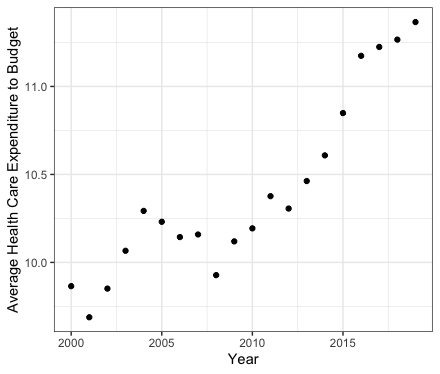
\includegraphics[width=0.8\textwidth]{figure/HealthCare_Point.png}	
\caption{Average ratio of Health Care Expenditure to Total Expenditure (Global)}
\end{figure}
\end{frame}

\begin{frame}
	\frametitle{Lawmakers}
	\begin{center}
	\alert{The proportion of seats held by female to the total seats count}	
\end{center}
	\begin{itemize}
		\item Lower house in Bicameral System
		\item Solo house in Unicameralism System
	\end{itemize}
	
	\begin{table}
\centering
\begin{tabular}{lllll} 
\hline
                     & Mean  & StD  & Min  & Max   \\ 
\hline
Global         & 19.66 & 11.64 & 0.00 & 63.75  \\
High Income Countries  & 27.36 & 9.94 & 7.08 & 47.6  \\
Emerging Market & 18.64  & 9.70 & 0.61 & 48.2  \\
LDC Countries   & 19.34 & 13.05 & 0.00 & 63.75 \\
\hline
\end{tabular}
\caption{Summary Statistics of Lawmakers (\%)}
\label{Health Care Summary}
\end{table}
\end{frame}

\begin{frame}[plain]
\begin{figure}
\centering
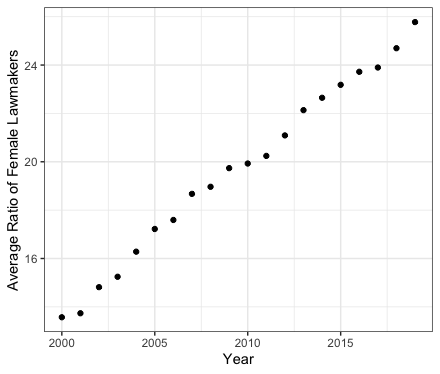
\includegraphics[width=0.8\textwidth]{figure/Lawmaker_Point.png}	
\caption{Average ratio of Female Lawmakers to Total Lawmakers (Global)}
\end{figure}
\end{frame}


\begin{frame}
	\frametitle{Control Variable}
	\begin{enumerate}
		\item Factors influence health care (\citeNP{Hitiris1992}\quad\citeNP{Gerdtham2000})
		\begin{itemize}
			\item Economic Development (GDP per capita)
			\item Demographic (Age group proportion)
			\item Contagious Disease (Number of Infections)
		\end{itemize}
		\item Foreign Aid
		\item Democracy
		\item Labour Participation Ratio: Better system or better gender \cite{Sung2003}
	\end{enumerate}
\end{frame}

\begin{frame}
	
\begin{table}[H]
\resizebox{\columnwidth}{!}{\begin{tabular}{lcccccccc}
\hline
                                                  &  & mean    &  & Std. deviation &  & min    &  & max      \\ \hline

GDP per capita (US\$)                             &  & 13401.4 &  & 18987.59       &  & 111.9  &  & 123514.2 \\
Age 64+ (\%)                               &  & 8.72    &  & 5.85           &  & 0.69   &  & 28.00    \\
Age 0-14 (\%)                               &  & 28.05    &  & 10.68           &  & 12.21   &  & 50.07    \\
TB cases (per 100,000 people)     &  & 131.7   &  & 201.31         &  & 0.00   &  & 1270.00  \\
Foreign Aid per capita (US\$) &  & 38.26   &  & 60.31          &  & -49.54 &  & 688.09   \\
Democracy index                                   &  & 0.67    &  & 0.25           &  & 0.05   &  & 0.98     \\
Female Labor Participation (\%)                   &  & 51.14   &  & 14.59          &  & 12.4   &  & 87.81    \\ \hline
\end{tabular}}
    \caption{The summary statistics of Control Variables}
    \label{Summary Statistics}
\end{table}
\end{frame}

\begin{frame}
	\frametitle{Binary Variables}
	\begin{itemize}
		\item Lawmaker Dummy: Annual Average
		\item Democracy Dummy: Demoracy or Autocracy
		\item Intersection
	\end{itemize}
\end{frame}

\begin{frame}
	\frametitle{Model}
	\begin{center}
		\alert{Fixed Effect Model}
	\end{center}
\vspace*{-1\baselineskip}
\begin{align*}
	HealthExp_{i,t} = \beta Lawmaker_{i,t-1} + \boldsymbol{\lambda}\mathbf{X}_{i,t} + \alpha_i + \gamma_t + \epsilon_{i,t}
\end{align*}
\vspace*{-1.2\baselineskip}
\begin{columns}
	\begin{column}{0.5\textwidth}
\begin{itemize}
\item $HealthExp_{i, t}$: Health Care Expenditure Ratio
\item $\mathbf{X}_{i,t}$: Control variables and Binary Variables
\item $\gamma_{t}$: Year Specific Fixed Effect
\item $i$: Country Indicator 1 - 122

\end{itemize}
	\end{column}
	\begin{column}{0.5\textwidth}  
		\begin{center}
\begin{itemize}
\item $Lawmaker_{i, t-1}$: Female Lawmaker Ratio (lag)
\item$\alpha_i$: Country Specific Fixed Effect
\item $\epsilon_{i,t}$: Turbulence Term
\item $t$: Year Indicator 2001 - 2019

\end{itemize}
		\end{center}
	\end{column}
\end{columns}
	
\end{frame}
%-------------------------------------------------------------------------------------------------------------------------------------------------------------------------------%
\section{Results}
\begin{frame}[plain]
\frametitle{Some Priliminary Results}
\begin{center}
	\begin{table}[]
\resizebox{\columnwidth}{!}{\begin{tabular}{lllllllll}
\hline
                                                  & (1)                                                               & (2)                                                                & (3)                                                               & (4)                                                                & (5)                                                               & (6)                                                               & (7)                                                               & (8)                                                               \\ \hline
Female Lawmaker (\%)                              & \begin{tabular}[c]{@{}l@{}}0.087$^{***}$\\ (0.003)\end{tabular}   & \begin{tabular}[c]{@{}l@{}}0.008\\ (0.009)\end{tabular}            & \begin{tabular}[c]{@{}l@{}}0.096$^{***}$\\ (0.004)\end{tabular}   & \begin{tabular}[c]{@{}l@{}}0.006\\ (0.009)\end{tabular}            & \begin{tabular}[c]{@{}l@{}}0.096$^{***}$\\ (0.004)\end{tabular}   & \begin{tabular}[c]{@{}l@{}}0.005\\ (0.01)\end{tabular}            & \begin{tabular}[c]{@{}l@{}}0.098$^{***}$\\ (0.004)\end{tabular}   & \begin{tabular}[c]{@{}l@{}}0.005\\ (0.009)\end{tabular}           \\
GDP per capita (US\$)                             & \begin{tabular}[c]{@{}l@{}}0.00003$^{***}$\\ (0.000)\end{tabular} & \begin{tabular}[c]{@{}l@{}}0.00004$^{***}$\\ (0.0000)\end{tabular} & \begin{tabular}[c]{@{}l@{}}0.00003$^{***}$\\ (0.000)\end{tabular} & \begin{tabular}[c]{@{}l@{}}0.00003$^{***}$\\ (0.0000)\end{tabular} & \begin{tabular}[c]{@{}l@{}}0.00003$^{***}$\\ (0.000)\end{tabular} & \begin{tabular}[c]{@{}l@{}}0.00003$^{***}$\\ (0.000)\end{tabular} & \begin{tabular}[c]{@{}l@{}}0.00001$^{***}$\\ (0.000)\end{tabular} & \begin{tabular}[c]{@{}l@{}}0.00003$^{***}$\\ (0.000)\end{tabular} \\
Population 64+ (\%)                               & \begin{tabular}[c]{@{}l@{}}0.146$^{***}$\\ (0.01)\end{tabular}    & \begin{tabular}[c]{@{}l@{}}0.317$^{***}$\\ (0.041)\end{tabular}    & \begin{tabular}[c]{@{}l@{}}0.172$^{***}$\\ (0.011)\end{tabular}   & \begin{tabular}[c]{@{}l@{}}0.271$^{***}$\\ (0.044)\end{tabular}    & \begin{tabular}[c]{@{}l@{}}0.172$^{***}$\\ (0.011)\end{tabular}   & \begin{tabular}[c]{@{}l@{}}0.258$^{***}$\\ (0.042)\end{tabular}   & \begin{tabular}[c]{@{}l@{}}-0.0001\\ (0.021)\end{tabular}         & \begin{tabular}[c]{@{}l@{}}0.264$^{***}$\\ (0.04)\end{tabular}    \\
Population 0-14 (\%)                              & \begin{tabular}[c]{@{}l@{}}-0.086$^{***}$\\ (0.013)\end{tabular}  & \begin{tabular}[c]{@{}l@{}}-0.275$^{***}$\\ (0.032)\end{tabular}   & \begin{tabular}[c]{@{}l@{}}-0.062$^{***}$\\ (0.013)\end{tabular}  & \begin{tabular}[c]{@{}l@{}}-0.261$^{***}$\\ (0.032)\end{tabular}   & \begin{tabular}[c]{@{}l@{}}-0.063$^{***}$\\ (0.013)\end{tabular}  & \begin{tabular}[c]{@{}l@{}}-0.259$^{***}$\\ (0.031)\end{tabular}  & \begin{tabular}[c]{@{}l@{}}-0.09$^{***}$\\ (0.017)\end{tabular}   & \begin{tabular}[c]{@{}l@{}}-0.257$^{***}$\\ (0.03)\end{tabular}   \\
Incident of Tuberculosis (per 100,000 people)     & \begin{tabular}[c]{@{}l@{}}-0.001$^{***}$\\ (0.0002)\end{tabular} & \begin{tabular}[c]{@{}l@{}}0.002$^{***}$\\ (0.0006)\end{tabular}   & \begin{tabular}[c]{@{}l@{}}-0.001$^{***}$\\ (0.0002)\end{tabular} & \begin{tabular}[c]{@{}l@{}}0.002$^{***}$\\ (0.0006)\end{tabular}   & \begin{tabular}[c]{@{}l@{}}-0.001$^{***}$\\ (0.0002)\end{tabular} & \begin{tabular}[c]{@{}l@{}}0.002$^{***}$\\ (0.0006)\end{tabular}  & \begin{tabular}[c]{@{}l@{}}-0.002$^{***}$\\ (0.0003)\end{tabular} & \begin{tabular}[c]{@{}l@{}}0.002$^{***}$\\ (0.0006)\end{tabular}  \\
Female Labor Participation (\%)                   &                                                                   &                                                                    & \begin{tabular}[c]{@{}l@{}}-0.028$^{***}$\\ (0.0034)\end{tabular} & \begin{tabular}[c]{@{}l@{}}0.067$^{***}$\\ (0.015)\end{tabular}    & \begin{tabular}[c]{@{}l@{}}-0.028$^{***}$\\ (0.003)\end{tabular}  & \begin{tabular}[c]{@{}l@{}}0.064$^{***}$\\ (0.015)\end{tabular}   & \begin{tabular}[c]{@{}l@{}}-0.031$^{***}$\\ (0.004)\end{tabular}  & \begin{tabular}[c]{@{}l@{}}0.065$^{***}$\\ (0.015)\end{tabular}   \\
Official Development Assistance per capita (US\$) &                                                                   &                                                                    &                                                                   &                                                                    & \begin{tabular}[c]{@{}l@{}}0.0009\\ (0.0008)\end{tabular}         & \begin{tabular}[c]{@{}l@{}}-0.005$^{***}$\\ (0.001)\end{tabular}  & \begin{tabular}[c]{@{}l@{}}-0.001$^{*}$\\ (0.0009)\end{tabular}   & \begin{tabular}[c]{@{}l@{}}-0.005$^{***}$\\ (0.001)\end{tabular}  \\
Democracy index                                   &                                                                   &                                                                    &                                                                   &                                                                    &                                                                   &                                                                   & \begin{tabular}[c]{@{}l@{}}5.743$^{***}$\\ (0.331)\end{tabular}   & \begin{tabular}[c]{@{}l@{}}0.689\\ (0.6)\end{tabular}             \\
Lawmaker Dummy                                    &                                                                   &                                                                    &                                                                   &                                                                    &                                                                   &                                                                   &                                                                   &                                                                   \\
Democracy Dummy                                   &                                                                   &                                                                    &                                                                   &                                                                    &                                                                   &                                                                   &                                                                   &                                                                   \\
Intersection Term                                 &                                                                   &                                                                    &                                                                   &                                                                    &                                                                   &                                                                   &                                                                   &                                                                   \\
Fixed Effect: Year                                & YES                                                               & YES                                                                & YES                                                               & YES                                                                & YES                                                               & YES                                                               & YES                                                               & YES                                                               \\
Fixed Effect: Country                             & NO                                                                & YES                                                                & NO                                                                & YES                                                                & NO                                                                & YES                                                               & NO                                                                & YES                                                               \\
Adjust $R^2$                                      & 0.339                                                             & 0.892                                                              & 0.346                                                             & 0.893                                                              & 0.346                                                             & 0.894                                                             & 0.402                                                             & 0.894                                                             \\ \hline
\end{tabular}}
\end{table}
\end{center}
\end{frame}

\begin{frame}[plain]
	\frametitle{Country Groups}
	\begin{center}
	
	\begin{table}[]
\resizebox{\columnwidth}{!}{\begin{tabular}{lllll}
\hline
                                                  & (1)                                                              & (2)                                                              & (3)                                                            & (4)                                                            \\ 
Country Group                                     & High Income                                                      & Emerging                                                         & LDC                                                            & LDC                                                            \\ \hline
Female Lawmaker (\%)                              & \begin{tabular}[c]{@{}l@{}}-0.068$^{***}$\\ (0.014)\end{tabular} & \begin{tabular}[c]{@{}l@{}}0.007\\ (0.019)\end{tabular}          & \begin{tabular}[c]{@{}l@{}}0.02\\ (0.018)\end{tabular}         & \begin{tabular}[c]{@{}l@{}}0.019\\ (0.018)\end{tabular}        \\
GDP per capita (US\$)                             & \begin{tabular}[c]{@{}l@{}}0.00003$^{**}$\\ (0.000)\end{tabular} & \begin{tabular}[c]{@{}l@{}}0.0001$^{*}$\\ (0.0000)\end{tabular}  & \begin{tabular}[c]{@{}l@{}}0.00003\\ (0.000)\end{tabular}      & \begin{tabular}[c]{@{}l@{}}0.00008\\ (0.0001)\end{tabular}     \\
Population 64+ (\%)                               & \begin{tabular}[c]{@{}l@{}}0.704$^{***}$\\ (0.063)\end{tabular}  & \begin{tabular}[c]{@{}l@{}}0.066\\ (0.097)\end{tabular}          & \begin{tabular}[c]{@{}l@{}}-1.48\\ (0.718)\end{tabular}        & \begin{tabular}[c]{@{}l@{}}-1.614$^{*}$\\ (0.705)\end{tabular} \\
Population 0-14 (\%)                              & \begin{tabular}[c]{@{}l@{}}0.608$^{***}$\\ (0.073)\end{tabular}  & \begin{tabular}[c]{@{}l@{}}-0.251$^{***}$\\ (0.035)\end{tabular} & \begin{tabular}[c]{@{}l@{}}-0.396$^{*}$\\ (0.146)\end{tabular} & \begin{tabular}[c]{@{}l@{}}-0.382$^{*}$\\ (0.145)\end{tabular} \\
Incident of Tuberculosis (per 100,000 people)     & \begin{tabular}[c]{@{}l@{}}0.033$^{**}$\\ (0.008)\end{tabular}   & \begin{tabular}[c]{@{}l@{}}-0.002$^{*}$\\ (0.001)\end{tabular}   & \begin{tabular}[c]{@{}l@{}}0.0005\\ (0.001)\end{tabular}       & \begin{tabular}[c]{@{}l@{}}0.0003\\ (0.001)\end{tabular}       \\
Female Labor Participation (\%)                   & \begin{tabular}[c]{@{}l@{}}0.038\\ (0.028)\end{tabular}          & \begin{tabular}[c]{@{}l@{}}-0.022\\ (0.021)\end{tabular}         & \begin{tabular}[c]{@{}l@{}}-0.006\\ (0.042)\end{tabular}       & \begin{tabular}[c]{@{}l@{}}0.001\\ (0.04)\end{tabular}         \\
Official Development Assistance per capita (US\$) &                                                                  &                                                                  &                                                                & \begin{tabular}[c]{@{}l@{}}0.005$^{\#}$\\ (0.002)\end{tabular}  \\
Fixed Effect: Year                                & YES                                                              & YES                                                              & YES                                                            & YES                                                            \\
Fixed Effect: Country                             & YES                                                              & YES                                                              & YES                                                            & YES                                                            \\
Adjust $R^2$                                      & 0.901                                                            & 0.941                                                            & 0.392                                                          & 0.396                                                          \\ \hline
\end{tabular}}
\end{table}
\end{center}
\end{frame}


%-------------------------------------------------------------------------------------------------------------------------------------------------------------------------------%

\section{Epilogue}

\begin{frame}
	\frametitle{Findings}
	\begin{enumerate}
		\item In general, no clear relationship between lawmaker's gender and health care expenditure. (\citeNP{Irma2011}'s finding)
		\item In well developed countries, negative influence existes. (Can't explain yet.)
		\item When reading similar papers, need more caution.
		\item Other factors are overpower 
	\end{enumerate}
\end{frame}

\begin{frame}
	\frametitle{Limitation and Plan}


\begin{columns}
	\begin{column}{0.5\textwidth}
\begin{itemize}
\item Limitation
		\begin{enumerate}
	\item Sample size: 122 $\times$ 19
	\item Handling missing value: better solution
	\item Better system measurement: robustness 
		\end{enumerate}
\end{itemize}
	\end{column}
	\begin{column}{0.5\textwidth}  

\begin{itemize}
\item Plan \& Extension
	\begin{enumerate}
		\item Implement the binary: DID (some flaws)
		\item Country's case studies
		\item If time allow: solve some limitations
		\item Consider the adminstration branch
	\end{enumerate}
\end{itemize}
	\end{column}
\end{columns}
	
\end{frame}

\begin{frame}
	\centering	
\huge{ Thanks for listening\\}
\end{frame}


%-------------------------------------------------------------------------------------------------------------------------------------------------------------------------------%
\begin{frame}[allowframebreaks]
	\frametitle{Bibliography}
	\bibliographystyle{apacite}

{\footnotesize\bibliography{export.bib}}
\end{frame}
\end{document}